\documentclass[11pt]{article}
\usepackage{graphicx}
\begin{document}

\begin{titlepage}

\begin{center}
\begin{huge}
Swarm Visualiser - COS 301 Main Project
\\
Design Specification- General Purpose Optimiser
\begin{small}
\\
Team: Dragon Brain
\\
Members:
\\
Matheu Botha u14284104
\\
Renton McInytre u14312710
\\
Emilio Singh u14006512
\\
Gerard van Wyk u14101263

\end{small}

\end{huge}
\end{center}
\end{titlepage}

\pagebreak

\tableofcontents
\pagebreak
\section{System Component: General Optimiser}
\subsection{Purpose}
\paragraph{The SwarmVis program is comprised of many separate parts. Crucial to the point of the visualisation, is the actual optimiser whose results need to be visualised. This is a service performed by the OPT Module which is described in this text.}

\subsection{Relation to System as a Whole}
\paragraph{The OPT module will perform whatever optimisation task it has been configured to do and then place its results, as they happen, into the Model component of the system. From there, the Graphical Pipeline will be responsible for rendering the results to the screen. The OPT module is largely independent of the other modules and the other modules, especially, are independent of it. The only interaction that occurs between the OPT module and the rest of the system is the user configuration mediated by the interface and the message passing from the OPT module to the Model module.
}
\subsection{Model}

\begin{figure}
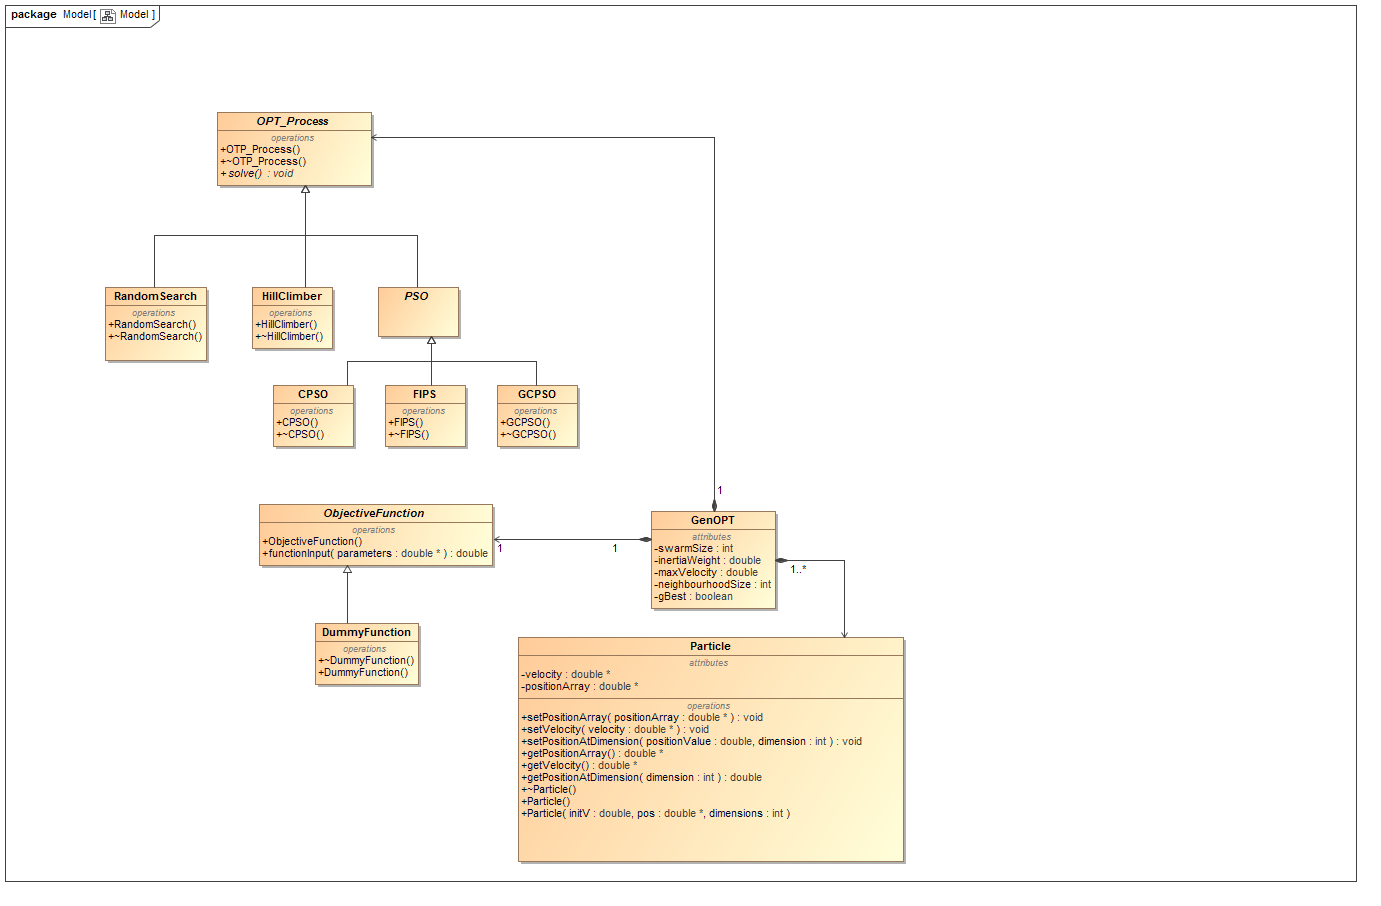
\includegraphics[scale=0.45]{Model.png}
\caption{The diagram presented above is the Model diagram explaining the structure of the OPT Module}
\end{figure}

\end{document}